\section{Desarrollo}\label{desarrollo}

\subsection{Exploración de Superficies de
Ataque}\label{exploraciuxf3n-de-superficies-de-ataque}

\begin{figure}
\centering
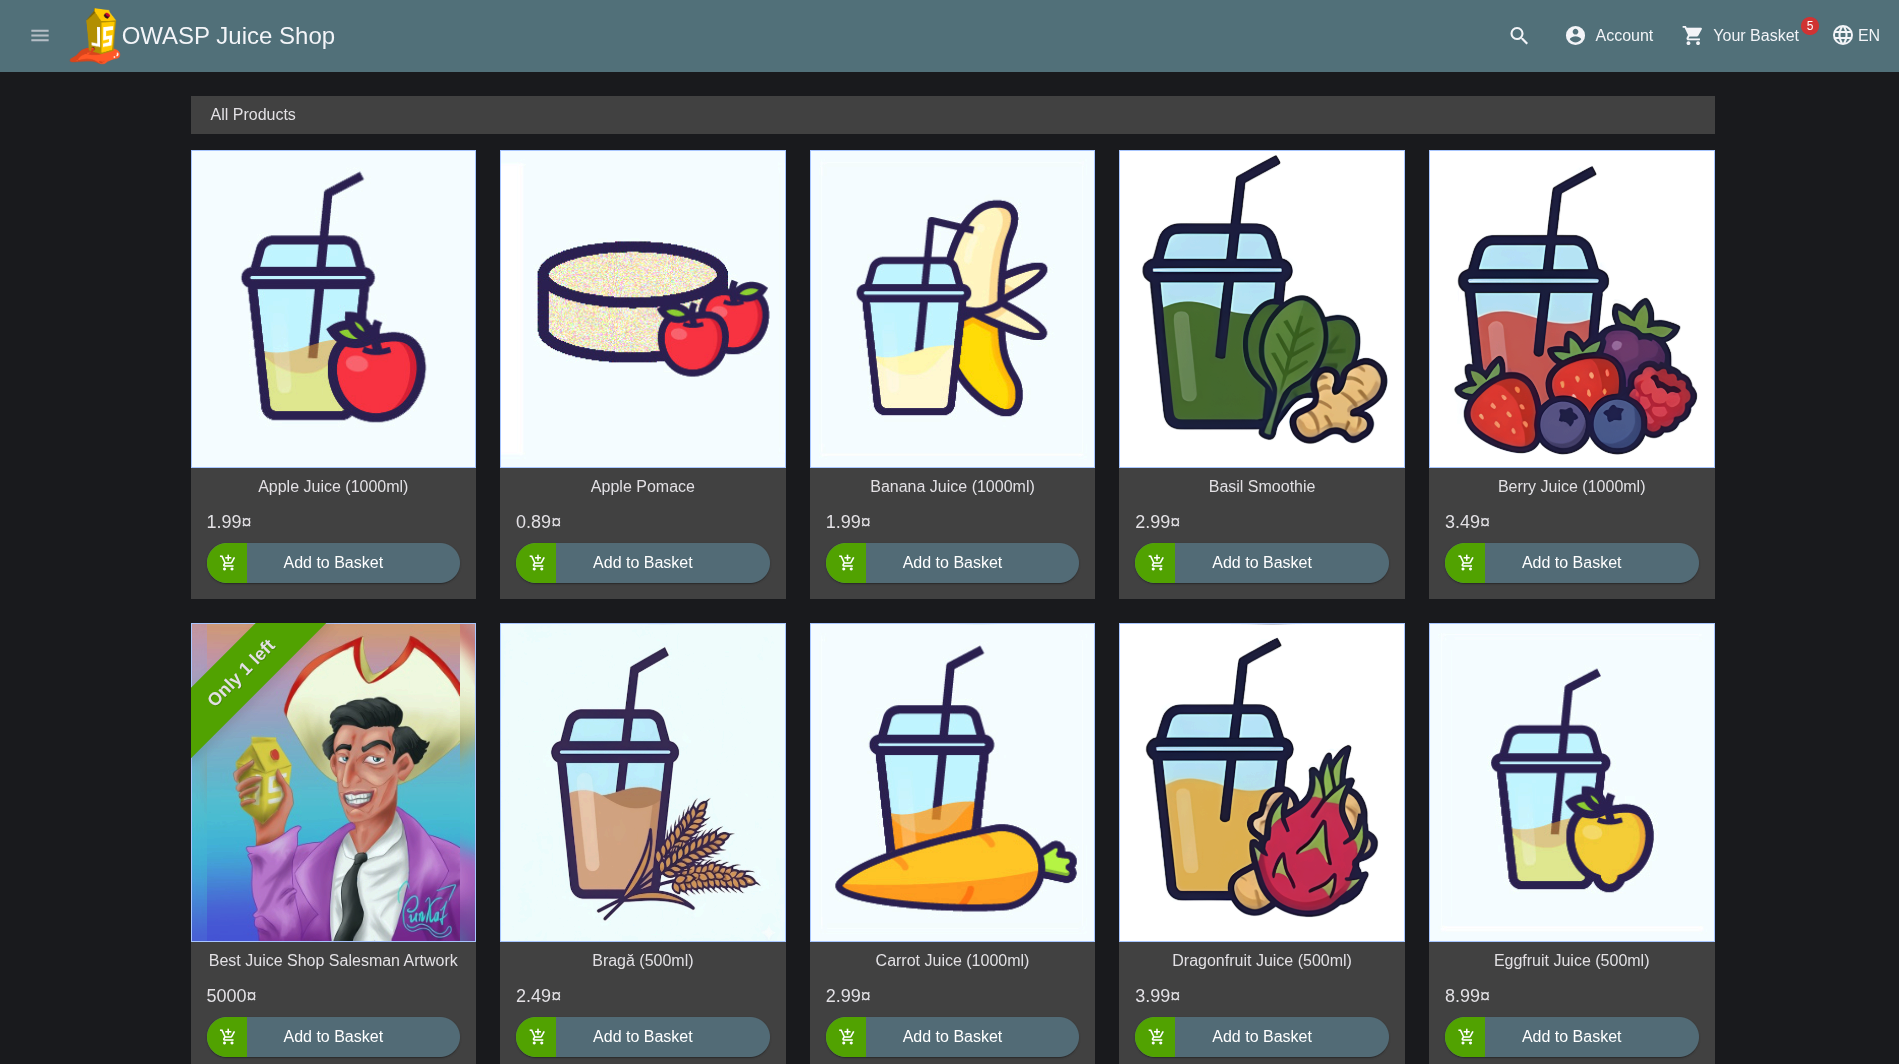
\includegraphics[keepaspectratio]{./img/startpage.png}
\caption{Página Inicial\label{startpage}}
\end{figure}

Al iniciar la aplicación, se pueden visualizar ciertos productos que se
enfocan en la venta de jugos, tal como se observa en la figura
\ref{startpage}. Esta página fue desarrollada por OWASP.

En esta página vulnerable, se pueden visualizar barras de búsqueda
(\ref{search}), formularios (\ref{form}) y autenticación (\ref{auth}).

\begin{figure}
\centering
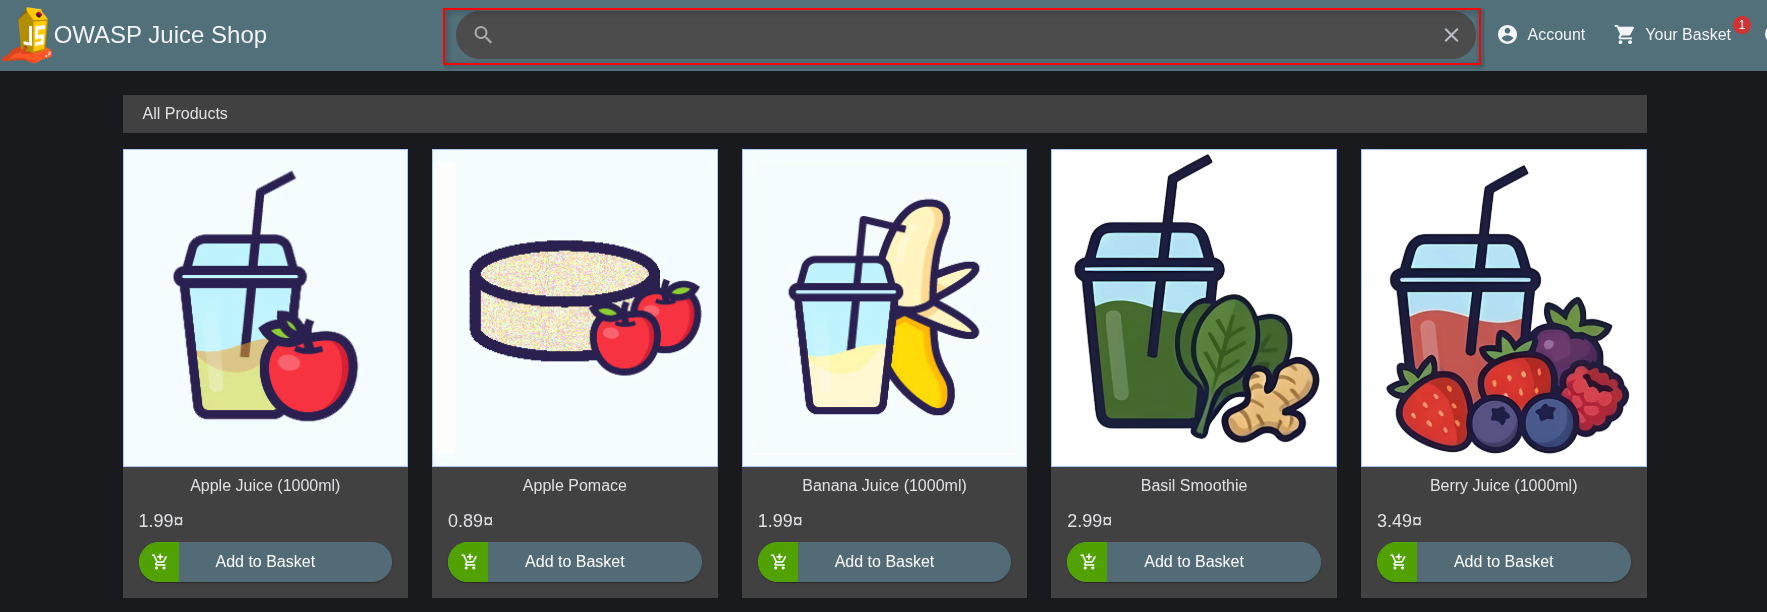
\includegraphics[keepaspectratio]{./img/search.png}
\caption{Barra de Búsqueda\label{search}}
\end{figure}

\begin{figure}
\centering
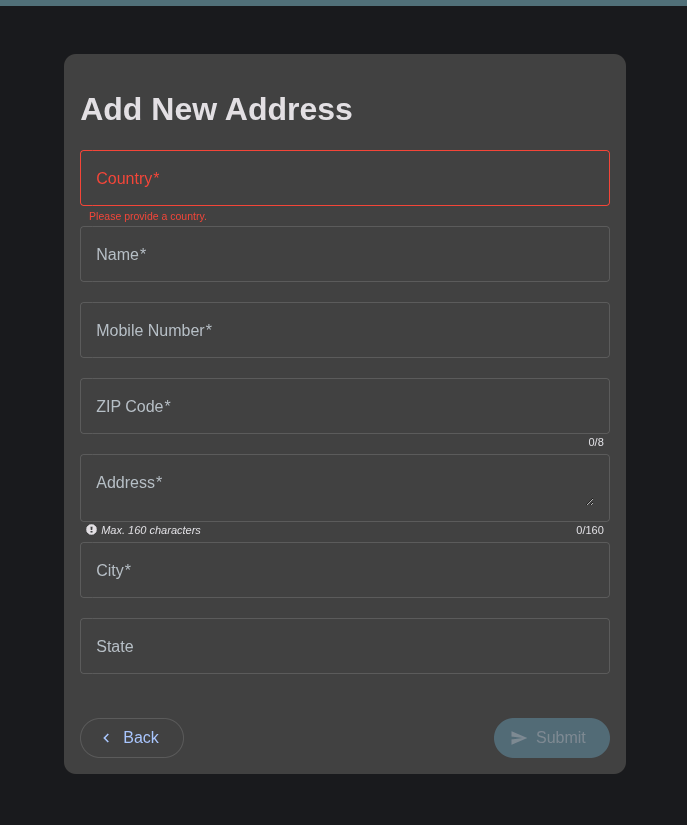
\includegraphics[keepaspectratio]{./img/form.png}
\caption{Formularios\label{form}}
\end{figure}

\begin{figure}
\centering
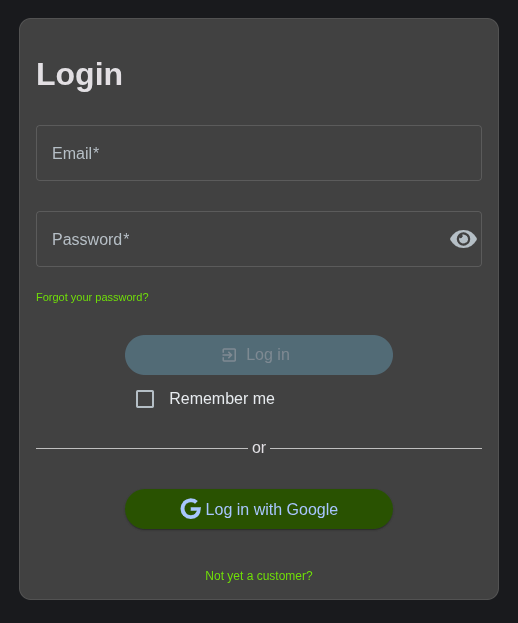
\includegraphics[keepaspectratio]{./img/auth.png}
\caption{Autenticación\label{auth}}
\end{figure}

Todos estos campos mostrados en las figuras \ref{search}, \ref{form} y
\ref{auth} muestran campos de texto, principalmente etiquetas HTML:

\begin{lstlisting}[language=HTML]
<input type="text" />
\end{lstlisting}

En todas estas es posible vulnerar el valor que se envía a estas
páginas.

\subsection{\texorpdfstring{\emph{SQL
Injection}}{SQL Injection}}\label{sql-injection}

Para complacer el taller especificado, se ingresarán ciertos valores
para comprobar si es posible vulnerar estos campos ingresando
instrucciones para el motor de base de datos. Esto con el fin de
comprobar qué datos se envían y cuáles están ocultos al usuario.

\subsubsection{\texorpdfstring{\emph{SQL Injection} en Barra de
Búsqueda}{SQL Injection en Barra de Búsqueda}}\label{sql-injection-en-barra-de-buxfasqueda}

\begin{figure}
\centering
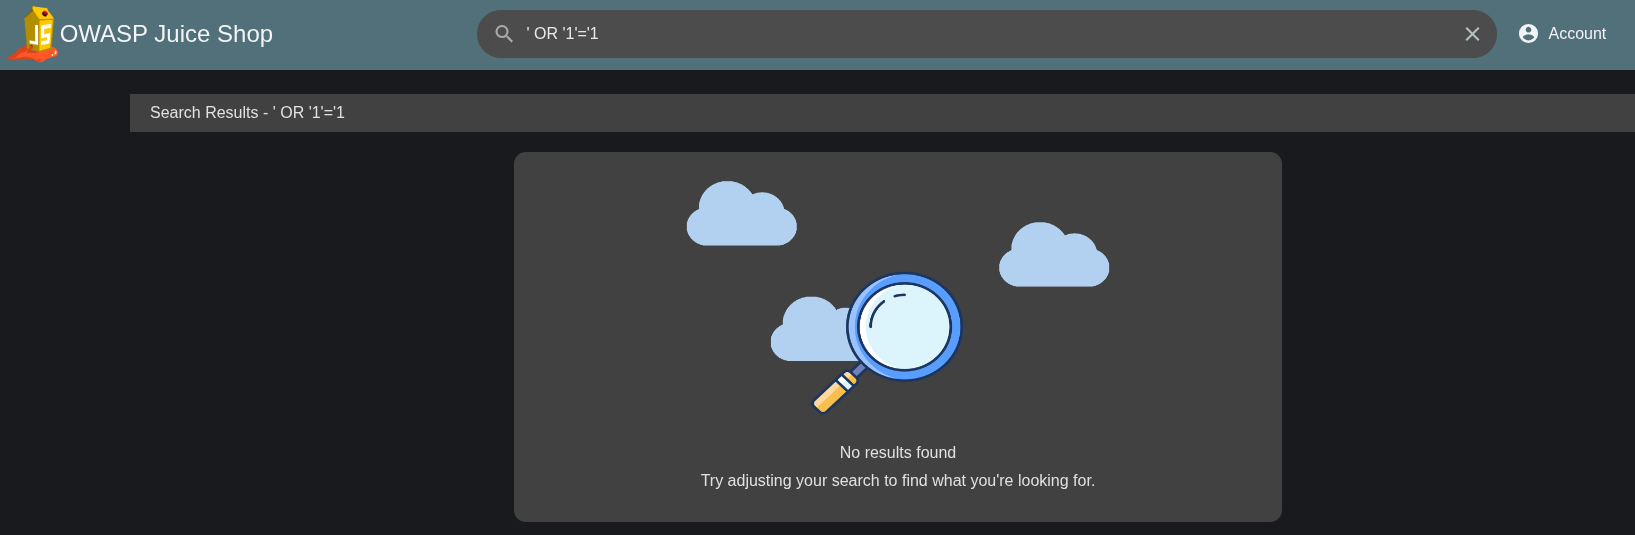
\includegraphics[keepaspectratio]{./img/search_sql.png}
\caption{Resultado de Inyección SQL en Barra de
Búsqueda\label{search_sql}}
\end{figure}

Tal como se observa en la figura \ref{search_sql}, no se logró vulnerar
completamente los productos y datos sensibles de usuarios.

Si existiese un error, lo ideal sería no trabajar directamente con SQL
dentro de la aplicación, sino un DTO.

\subsection{Cross-Site Scripting (XSS)}\label{cross-site-scripting-xss}

Este tipo de ataque consiste en ingresar un \emph{script} dentro de la
página web que permita ejecutar cierto código malicioso. Esta página es
insegura debido a que, como se observa en la figura \ref{alert_xss}, se
pueden ejecutar algunos comandos dentro de la página.

\begin{figure}
\centering
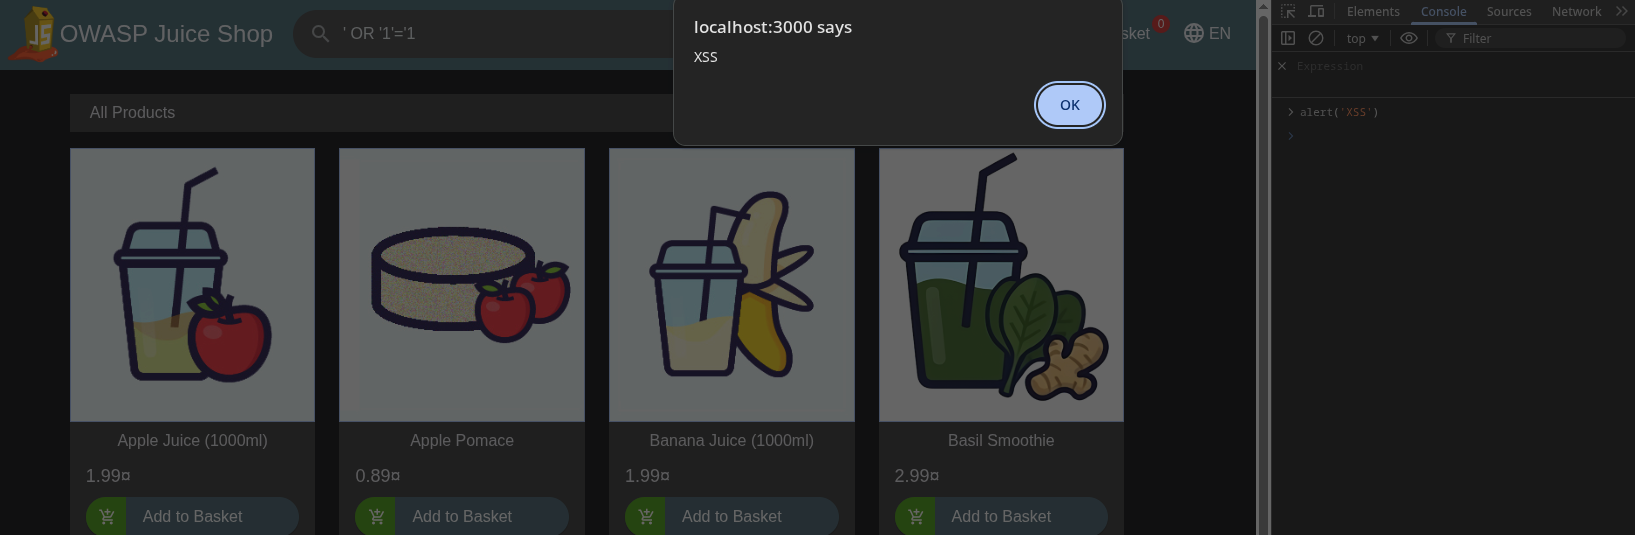
\includegraphics[keepaspectratio]{./img/alert_xss.png}
\caption{Ejecución de \emph{script} malicioso\label{alert_xss}}
\end{figure}

\subsection{Configuración Insegura}\label{configuraciuxf3n-insegura}

Ya que la imagen fue instanciada en Docker, no se tiene un \emph{shell}
especializado para revisar los archivos de configuración. Sin embargo,
es posible acceder a la API REST sin necesidad de validación de usuario,
tal como se observa en la figura \ref{api_products}.

\begin{figure}
\centering
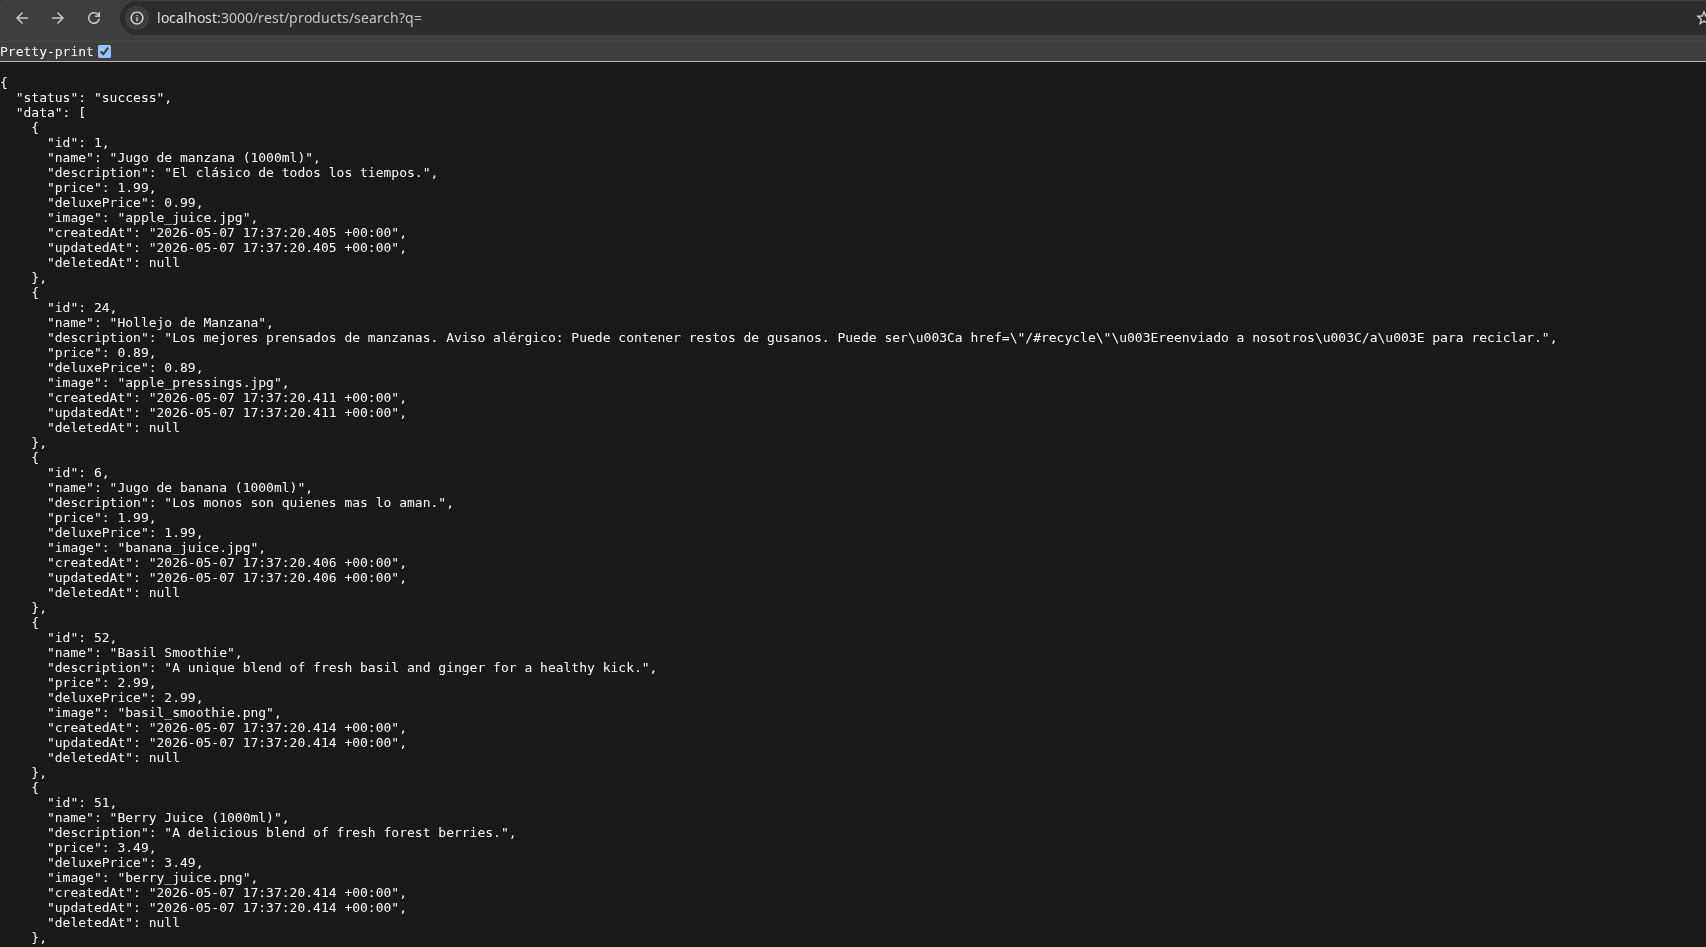
\includegraphics[keepaspectratio]{./img/api_products.png}
\caption{Respuesta de API de los productos\label{api_products}}
\end{figure}

\begin{figure}
\centering
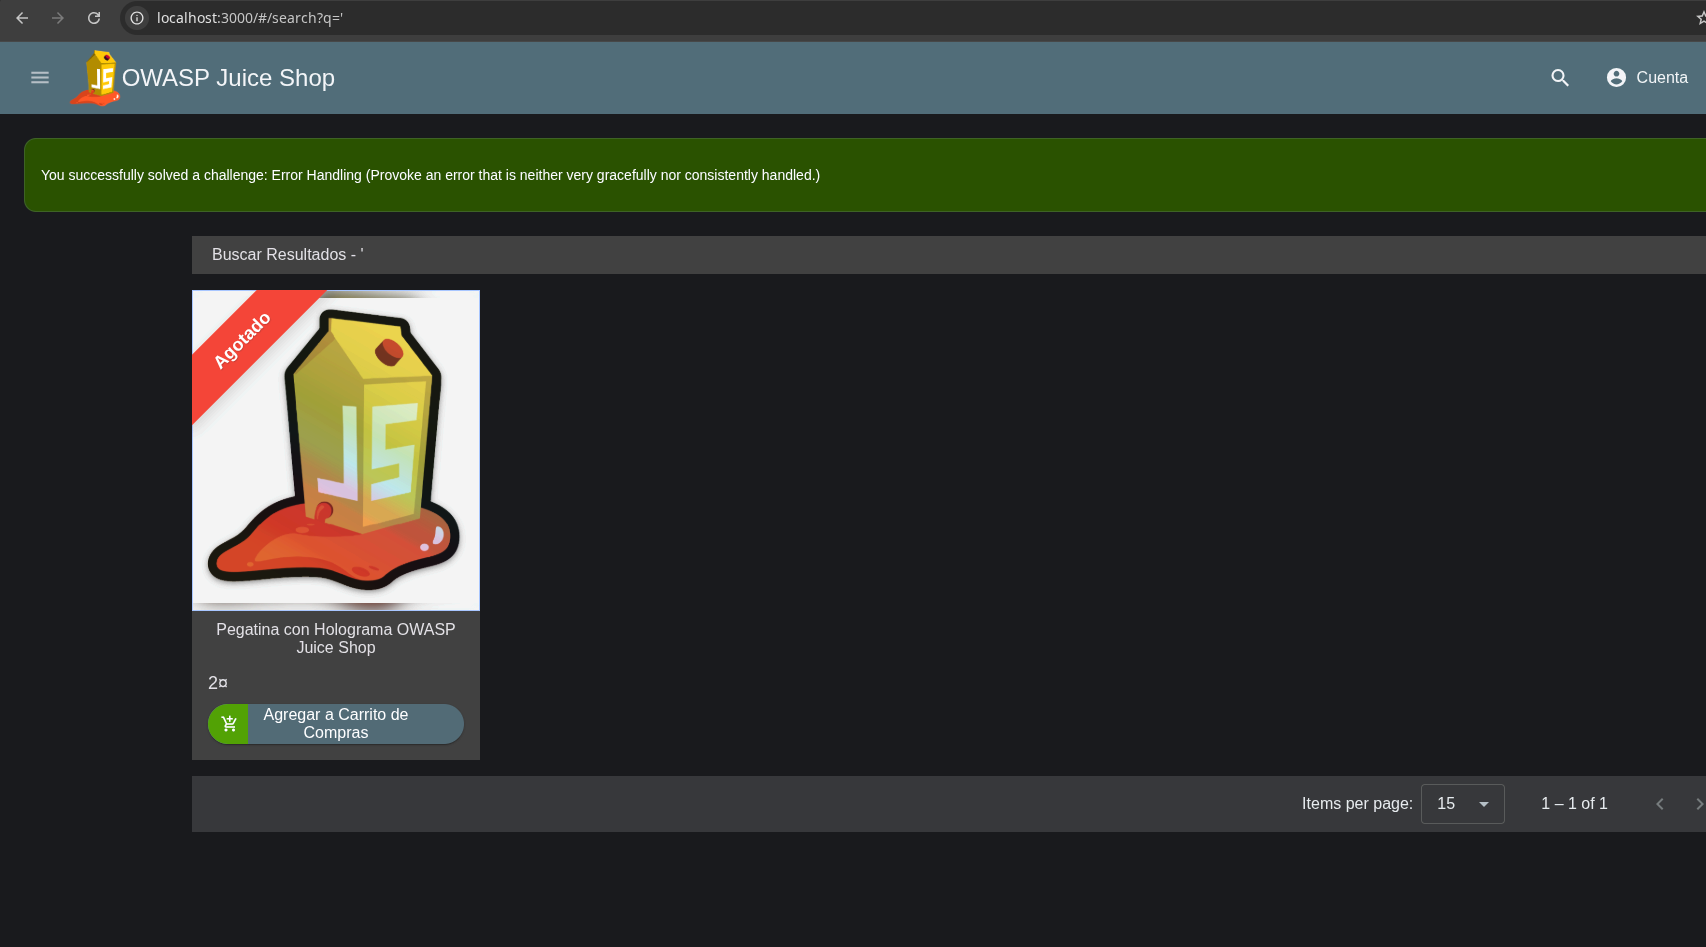
\includegraphics[keepaspectratio]{./img/products_hidden.png}
\caption{Productos ocultos o sin disponibilidad\label{products_hidden}}
\end{figure}

Además, se pueden visualizar algunos productos ocultos los cuales son
parte de un error. En la figura \ref{products_hidden} se observan los
productos que han sido descartados. Además, se puede apreciar un error
encontrado dentro de la página, el cual estaba destinado a ser
encontrado.
